\documentclass[a4paper,12pt, oneside]{book}

% \usepackage{fullpage}
\usepackage[italian]{babel}
\usepackage[utf8]{inputenc}
\usepackage{amssymb}
\usepackage{amsthm}
\usepackage{graphics}
\usepackage{amsfonts}
\usepackage{listings}
\usepackage{amsmath}
\usepackage{amstext}
\usepackage{engrec}
\usepackage{rotating}
\usepackage{verbatim}
\usepackage[safe,extra]{tipa}
\usepackage{showkeys}
\usepackage{multirow}
\usepackage{hyperref}
\usepackage{microtype}
\usepackage{fontspec}
\usepackage{enumerate}
\usepackage{braket}
\usepackage{marginnote}
\usepackage{pgfplots}
\usepackage{cancel}
\usepackage{polynom}
\usepackage{booktabs}
\usepackage{enumitem}
\usepackage{framed}
\usepackage{pdfpages}
\usepackage{pgfplots}
\usepackage{algorithm}
% \usepackage{algpseudocode}
\usepackage[cache=false]{minted}
\usepackage{mathtools}
\usepackage[noend]{algpseudocode}
\usepackage{varwidth,pst-tree,realscripts}
\usepackage{bidi}
\usetikzlibrary{automata,positioning}
\psset{showbbox=false,treemode=D,linewidth=0.3pt,treesep=2ex,levelsep=0.5cm}
\newcommand{\LFTw}[2]{%
\Tr[ref=#1]{\psframebox[linestyle=none,framesep=4pt]{%
\begin{varwidth}{15ex}\center #2\end{varwidth}}}}
\newcommand{\LFTr}[2]{\Tr[ref=#1]{\psframebox[linestyle=none,framesep=4pt]{#2}}}

\def\pstreehooki{\psset{thislevelsep=*0pt}}
\def\pstreehookiii{\psset{thislevelsep=*0pt}}
\def\pstreehookv{\psset{thislevelsep=*0pt}}

\usepackage{fancyhdr}
\pagestyle{fancy}

\fancyfoot[C]{\thepage}


\title{Metodi Formali\\
\large{Esercizi prima settimana}}
\author{Davide Cozzi, 829827}
\date{}

\pgfplotsset{compat=1.13}
\begin{document}
\maketitle

\definecolor{shadecolor}{gray}{0.80}
\setlist{leftmargin = 2cm}
\newtheorem{teorema}{Teorema}
\newtheorem{definizione}{Definizione}
\newtheorem{esempio}{Esempio}
\newtheorem{corollario}{Corollario}
\newtheorem{lemma}{Lemma}
\newtheorem{osservazione}{Osservazione}
\newtheorem{nota}{Nota}
\newtheorem{esercizio}{Esercizio}
\algdef{SE}[DOWHILE]{Do}{doWhile}{\algorithmicdo}[1]{\algorithmicwhile\ #1}

\renewcommand{\chaptermark}[1]{%
  \markboth{\chaptername
    \ \thechapter.\ #1}{}}
\renewcommand{\sectionmark}[1]{\markright{\thesection.\ #1}}
\newcommand{\floor}[1]{\lfloor #1 \rfloor}
\section*{Esercizio 1}
Dato il sistema in figura stabilire insieme dei casi raggiungibili e
l'insieme dei passi, infine disegnare il grafo dei casi raggiungibili:
\begin{figure}[H]
  \centering
  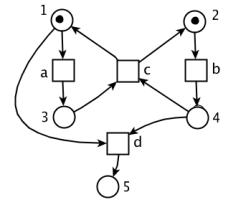
\includegraphics[scale = 0.6]{img/1.jpg}
\end{figure}
Si ha che:
\begin{itemize}
  \item l'\textit{insieme dei casi raggiungibili} è:
  \[C_\Sigma = \Big\{ \{1,2\},\{3,2\}, \{1,4\}, \{3,4\},
    \{5,2\},\{1,5\}\Big\}\]
  \item l'\textit{insieme dei passi} è:
  \[U_\Sigma = \Big\{ \{a\},\{b\}, \{c\}, \{d\}, \{a,b\}\Big\}\]
\end{itemize}
Si ha quindi il \textit{grafo dei casi}:
\begin{center}
  \begin{tikzpicture}[shorten >=1pt,node distance=3.41cm,on grid,auto]
    \node[] (q_0) {$\{5,2\}$};
    \node[] (q_1) [below=of q_0] {$\{1,2\}$};
    \node[] (q_2) [below left=of q_1] {$\{3,2\}$};
    \node[] (q_3) [below right=of q_1] {$\{1,4\}$};
    \node[] (q_4) [below right=of q_2] {$\{3,4\}$};
    \node[] (q_5) [right=of q_3] {$\{1,5\}$};
    \path[->]
    (q_1) edge node {$\{d\}$} (q_0)
    edge node [above left] {$\{a\}$} (q_2)
    edge node {$\{b\}$} (q_3)
    edge [bend right = 25] node [left] {$\{a,b\}$} (q_4)
    (q_2) edge node [below left] {$\{b\}$} (q_4)
    (q_3) edge node {$\{a\}$} (q_4)
    edge node {$\{d\}$} (q_5)
    (q_4) edge [bend right = 25] node [right] {$\{c\}$} (q_1)
    ;
  \end{tikzpicture}
\end{center}
\newpage
\section*{Esercizio 2}
Dati i due sistemi elementari in figura stabilire se sono isomorfi:
\begin{figure}[H]
  \centering
  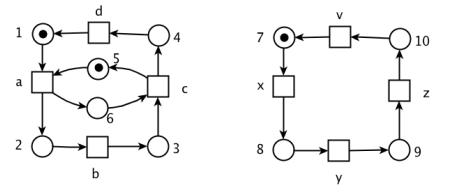
\includegraphics[scale = 0.6]{img/2.jpg}
\end{figure}
Disegno i due grafi dei casi sequenziali corrispondenti ai due sistemi:
\begin{enumerate}
  \item per il primo sistema:
  \begin{center}
    \begin{tikzpicture}[shorten >=1pt,node distance=3cm,on grid,auto]
      \node[] (q_1) {$\{1,5\}$};
      \node[] (q_2) [below left=of q_1] {$\{2,6\}$};
      \node[] (q_3) [below right=of q_1] {$\{4,5\}$};
      \node[] (q_4) [below right=of q_2] {$\{3,6\}$};
      \path[->]
      (q_1) edge node [above left] {$\{a\}$} (q_2)
      (q_2) edge node [below left] {$\{b\}$} (q_4)
      (q_4) edge node [below right] {$\{c\}$} (q_3)
      (q_3) edge node [above right] {$\{d\}$} (q_1)
      ;
    \end{tikzpicture}
  \end{center}
  \item per il secondo sistema:
  \begin{center}
    \begin{tikzpicture}[shorten >=1pt,node distance=3cm,on grid,auto]
      \node[] (q_1) {$\{7\}$};
      \node[] (q_2) [below left=of q_1] {$\{8\}$};
      \node[] (q_3) [below right=of q_1] {$\{9\}$};
      \node[] (q_4) [below right=of q_2] {$\{10\}$};
      \path[->]
      (q_1) edge node [above left] {$\{x\}$} (q_2)
      (q_2) edge node [below left] {$\{y\}$} (q_4)
      (q_4) edge node [below right] {$\{z\}$} (q_3)
      (q_3) edge node [above right] {$\{v\}$} (q_1)
      ;
    \end{tikzpicture}
  \end{center}
\end{enumerate}
Posso quindi trovare due mappe biunivoche $\alpha$ e $\beta$ che mi permettono
di passare dagli stati e dagli eventi del primo sistema a quelli del secondo: i
due sistemi hanno quindi grafo dei casi isomorfi
\newpage
\section*{Esercizio 3}
Dato il sistema in figura calcolo il grafo dei casi raggiungibili:
\begin{figure}[H]
  \centering
  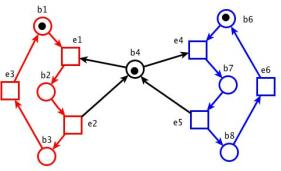
\includegraphics[scale = 0.7]{img/3.jpg}
\end{figure}
Si ottiene:
\begin{center}
  \begin{tikzpicture}[shorten >=1pt,node distance=3.8cm,on grid,auto]
    \node[] (q_1) {$\{b_1,b_4,b_6\}$};
    \node[] (q_4) [below right=of q_1] {$\{b_1,b_7\}$};
    \node[] (q_5) [below left=of q_1] {$\{b_2,b_6\}$};
    \node[] (q_2) [below =of q_5] {$\{b_3,b_4,b_6\}$};
    \node[] (q_3) [below =of q_4] {$\{b_1,b_4,b_8\}$};
    \node[] (q_6) [below =of q_2] {$\{b_3,b_7\}$};
    \node[] (q_7) [below =of q_3] {$\{b_2,b_8\}$};
    \node[] (q_8) [below right =of q_6] {$\{b_3,b_4,b_8\}$};
    \path[->]
    (q_1) edge node [above left] {$\{e_1\}$} (q_5)
    (q_1) edge node [above right] {$\{e_4\}$} (q_4)
    (q_5) edge node [left] {$\{e_2\}$} (q_2)
    (q_4) edge node [right] {$\{e_5\}$} (q_3)
    (q_2) edge node [below right] {$\{e_3\}$} (q_1)
    (q_3) edge node [below left] {$\{e_6\}$} (q_1)
    (q_3) edge node [right] {$\{e_1\}$} (q_7)
    (q_7) edge node [] {$\{e_2\}$} (q_8)
    (q_2) edge node [left] {$\{e_4\}$} (q_6)
    (q_6) edge node [below left] {$\{e_5\}$} (q_8)
    (q_8) edge node [above right] {$\{e_6\}$} (q_2)
    (q_8) edge node [above left] {$\{e_3\}$} (q_3)
    (q_7) edge [bend right = 10] node [right] {$\{e_6\}$} (q_5)
    (q_6) edge [bend left = 10] node [left] {$\{e_3\}$} (q_4)
    ;
  \end{tikzpicture}
\end{center}
\end{document}
% LocalWords:  img jpg above left node edge right of below bend distance
